\title{%
  \textbf{Interactive Tool for Teaching Hindley-Milner Type Inference through Visualisation}
  \\
  \Large{Progress report\\~\\~\textbf{Adam Jones}\\~Department of Computer Science\\~University of Warwick}
}

\documentclass[a4paper,fleqn,12pt]{article}

\usepackage[]{geometry}
\usepackage[utf8]{inputenc}
\usepackage[UKenglish]{babel}
\usepackage[UKenglish]{isodate}
\usepackage{amsmath}
\usepackage{amsfonts}
\usepackage{amssymb}
\usepackage{amsthm}
\usepackage{graphicx}
\usepackage{chngpage}
\usepackage{calc}
\PassOptionsToPackage{hyphens}{url}
\usepackage{hyperref}
\usepackage[nameinlink]{cleveref}
\usepackage{fancyhdr}
\usepackage{titletoc}
\usepackage[explicit]{titlesec}
\usepackage{natbib}
\usepackage[dvipsnames]{xcolor}
\usepackage[sc]{mathpazo}
\linespread{1.05} 
\usepackage[T1]{fontenc}
\usepackage{minted}
\usepackage{ragged2e}
\usepackage{adjustbox}
\definecolor{cs310lightgrey}{rgb}{0.95,0.95,0.95}
\usepackage[backgroundcolor=cs310lightgrey,hidealllines=true]{mdframed}

\hypersetup{
	colorlinks=true,
	linkcolor=black,
	urlcolor=black,
	citecolor=black
}

\BeforeBeginEnvironment{minted}{\begin{mdframed}}
\AfterEndEnvironment{minted}{\end{mdframed}}

\let\parencite\citep

\setlength{\parindent}{0mm}
\setlength{\parskip}{\medskipamount}
\renewcommand\baselinestretch{1.2}

\cleanlookdateon

\pagestyle{plain}
\renewcommand{\headrulewidth}{0.0pt}

\makeatletter
\fancypagestyle{plain}{
	\fancyhf{}
	\fancyhead[RE,RO]{\thepage}
	\fancyhead[LE,LO]{\textit{Interactive Tool for Teaching HM Type Inference through Visualisation}}
}
\makeatother

\begin{document}

\makeatletter
\begin{titlepage}

\LARGE \@title \\
\Large \\[1.5cm]

\vfill 

\begin{adjustwidth}{-\oddsidemargin-1in}{-\rightmargin}
  \centering
  
\includegraphics[width=\paperwidth]{line.png}
\end{adjustwidth}

\vspace*{-3.5cm}

\end{titlepage}
\makeatother

\pagestyle{plain}

\section{Introduction}\label{id:h.6k9gcmunzldy}

Static type checking identifies errors in programs at compile time, preventing runtime errors. Additionally, it allows for better tooling that improves developer productivity. For example, IDEs may use type information to suggest and perform automated refactorings \citep{ref1}.

However, specifying types manually (such as through annotations) can be time-consuming and potentially difficult. A type inference algorithm for a particular programming language’s type system can determine types automatically, which improves productivity by allowing programmers to get the best of types without having to explicitly specify them. Because of this, type inference is used in many popular programming languages with expressive type systems including Haskell, Rust and TypeScript.

An understanding of type inference would help computer scientists write cleaner code and debug type errors. However, few universities have core modules on type systems (although they may be touched on in programming curriculums, particularly functional programming modules) and there are limited easy-to-understand teaching resources on type inference. Therefore, many computer science graduates will be missing a useful understanding of how type inference actually works.

Hindley-Milner is a typed $\lambda$-calculus which allows for the types of programs in this calculus to be inferred and no type annotations are required \citep{ref2,ref3}. Various algorithms are available to infer these types such as Algorithm W by~\cite{ref3} and Algorithm M by~\cite{ref5}. Algorithm W takes a bottom-up approach, attempting to unify the types of subexpressions up the abstract syntax tree, while Algorithm M takes a top-down approach, unifying types down the tree. Both systems sometimes produce poor type error messages; Algorithm W often detects errors late, highlighting too large of a subexpression to be useful and Algorithm M often detects too specific of a term without context as to what original definition it violates. Because of this, hybrid or constraint-based algorithms along with heuristics are used in practice to provide more informative error messages. Despite not being required, explicit type annotations are often used to help identify errors earlier at locations which are easier to interpret \citep{ref6}.

Some programming languages including Haskell and ML (which OCaml and F\# are related to) have type systems that are originally based on Hindley-Milner, making it relevant for computer scientists to learn about today.

This project will deliver an interactive, web-based tool to help teach undergraduate students how Hindley-Milner type inference works. It will allow a student to type in an expression and see the steps of a type inference algorithm. This would be particularly useful in the context of modules teaching functional languages such as Haskell which perform similar type inference.

There is good evidence that this tool will be a useful teaching resource.~\cite{ref7} found in teaching the University of Porto’s functional programming course that “[presenting] the basis of type inference technology [...] significantly improved the way students deal with type errors because they understand the type system.” After implementing a successful teaching tool for visualising lambda-calculus parse trees,~\cite{ref8} noted that extending these to show type inference would have pedagogical value.

\subsection{Related work}\label{id:h.2mwaav7jkal4}

TypeTool by~\cite{ref7} was a tool that visualised type inference. It did this through a web application and was found to be beneficial for teaching purposes. However, it is inaccessible as the server hosting the application is no longer running and the source code has not been published. Additionally, as the parsing and type inference was done server-side there was a delay between the user entering an expression and seeing the result.

\cite{ref10} developed a visual functional programming system which visualises types during function application for a subset of Standard ML, used to teach first year undergraduate students. However, this did not explicitly show the type inference process and as a desktop application it is less accessible to lecturers and students. It also didn’t support key functional language constructs such as function declarations and let bindings.

These tools both use visualisation to help teach students about type systems in relation to functional programming. They allow users to enter their own expressions, so users can explore how the systems work in different cases to gain an intuitive understanding of the concepts. This interactive approach improves understanding as users can easily try testing their own assumptions or examine edge cases they are unsure of.

\section{Objectives}\label{id:h.qre9waa7e9so}

The ultimate goal of the project is to improve students’ knowledge and understanding of how type inference works. To achieve this, I will develop a resource for teaching Hindley-Milner type inference concepts to undergraduate students. A web application will allow students to enter expressions and view the results of a type inference algorithm, along with the steps taken to get to that result.

The three key parts of the project are the:

\begin{itemize}
  \item lexer and parser, to transform an entered expression into an abstract syntax tree
  \item type inference algorithm which operates on an abstract syntax tree to output steps taken and the final expression type
  \item web application to accept user input (the expression) and display the output from the type inference algorithm (the inferred type and process)
\end{itemize}

\subsection{Expression lexer and parser}\label{id:h.v6vafhv28y3i}

The first step in processing user input is lexing and parsing the expression they have entered. Lexing involves scanning the input string and exporting a sequence of tokens, while parsing takes this sequence of tokens and generates an abstract syntax tree (AST) from it.

Most type inference algorithms are designed to work on ASTs, as they are a commonly used theoretical representation of programs. Hence being able to generate an AST for a given input should allow for extending the project more easily. Additionally, representing a program as an AST is easy to extend if the language needs to be changed, as new types of tree nodes can be added without having to change the whole tree structure.

There is now a concrete vision for the expression language which includes variables, primitives, function application, function declarations and let bindings. Some other language constructs such as if-else conditional statements will be implemented as specialisations of other language features such as function application.

A basic lexer and recursive descent parser that supports some of these language features has been implemented, along with models to represent the AST nodes. This has put into practice skills from CS325 Compiler Design, which I am taking alongside the project in term 1. However, to fully implement the language I am considering rewriting the parser using a parser-combinator library such as Parjs \citep{ref11} or masala-parser \citep{ref12} as I have found manually writing a parser by hand is difficult, error-prone and time-consuming. Although, given my lack of any experience with parser combinators this approach may not necessarily be easier.

The lexer and parser are implemented in TypeScript, which compiles to JavaScript, as it will allow the entire application to run in a browser.

Compared to using a remote server, running the application in the browser avoids network requests which reduces operating costs and eliminates security vulnerabilities on the server related to accepting arbitrary code. This usually also runs faster as the browser does not have to wait for a response from the server. However on some devices (particularly those with less compute power like mobile phones) running the parser or type inference algorithm on large or pathological inputs may be slower than a server-client model.

As a statically-typed language TypeScript offers the benefits of static typing mentioned previously, improving productivity in the medium and long term. However, setting up TypeScript tooling took longer and as it requires compilation there is a longer delay between writing and running code than JavaScript. Additionally while TypeScript performs some type inference, it does not support complete type inference and therefore sometimes requires me to specify complex types explicitly which can be difficult.

\subsection{Type inference algorithm}\label{id:h.el6sta7fzq4a}

Key to the project is implementing the type inference algorithm. There are many such algorithms published, but the original one by~\cite{ref3}, Algorithm W, is being focused on. Understanding Algorithm W (and type systems more widely) has involved significant amounts of reading alongside weekly discussions with my supervisor.

Algorithm W and its dependencies (unification and substitution combination) have been successfully implemented in TypeScript. It accepts an abstract syntax tree as generated by the parser and outputs the final type of the expression. To ensure correctness and enable refactoring it has a significant test suite, including custom alpha-equivalence equality test matchers, for example:

\begin{minted}[breaklines]{js}
expect(e('[]')).toHaveType(list(a));
expect(e('cons', 'myNumber', '[]')).toHaveType(list(number));
expect(e('++', '[]', '[]')).toHaveType(list(a));
expect(e('uncons', '[]')).toHaveType(maybe(tuple(a, list(a))));
\end{minted}

This has been packaged as a self-contained npm module, separate from the language and web application projects. This helps decouple the components of the project, so they can be worked on somewhat independently and can be swapped out later. This could be useful if the project was extended in future to visualise other type inference algorithms for example. However, this does come with some extra complexity in publishing the different parts of the project and integrating them together.

Emitting the steps the algorithm is taking has not been completed yet. This will be a key step in the project as displaying steps taken will greatly aid understanding how the algorithm (and type inference more generally) works, contributing to the ultimate goal of the project.

\subsection{Web application}\label{id:h.cwlbt58wsbeg}

Finally, the deliverable that users will directly interact with is the web application. This will allow them to enter an expression, and send it through the lexer, parser and type inference algorithm. The results will then be displayed back to the user, showing the steps the type inference algorithm took.

A basic web application has been written in TypeScript, using the React framework. Using React helps with state management, should improve productivity and make testing considerably easier. Additionally, if the project is extended with more algorithms it will be possible to reuse components and be generally nicer to refactor. This does add to the page size and in turn loading times, although most of the bundle size is the project code itself so this is not a significant concern at the moment.

{\centering \begin{figure}[h!]
  \centering
  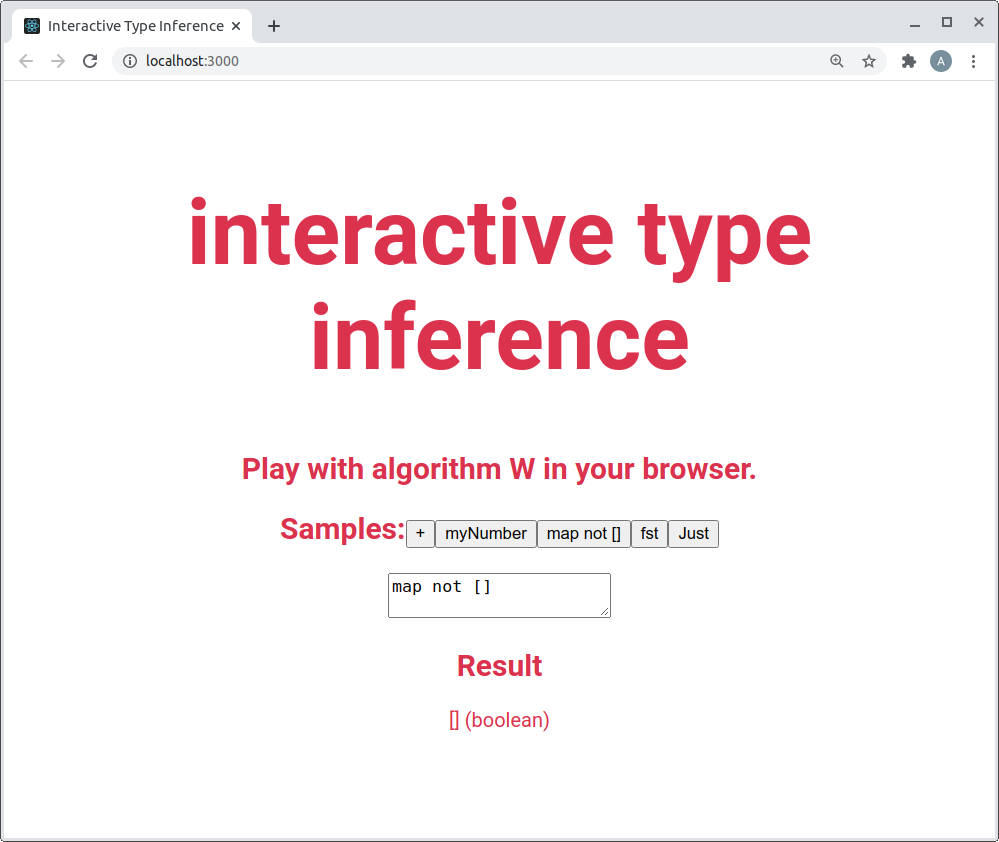
\includegraphics[width=0.818\linewidth]{images/image1.png}
  \caption{The web application showing the result of running algorithm W on an expression}
\end{figure} \par}

Given the limitations in the current parser and type inference algorithm it cannot parse all expressions in a user-friendly way and does not show the steps taken. However, it does demonstrate the various components working with each other in the browser to return a final result.

The application will be trialed with students to determine whether it is an effective teaching aid. This would likely involve showing them the application, explaining what it does and seeing how they use it, and testing whether they have a better understanding of type inference afterwards. Their feedback could be used to improve the application, and be valuable for the evaluation in the final report.

\section{Methods}\label{id:h.em0ria5zbf4p}

\subsection{Research process}\label{id:h.ew85fk610kqt}

I have maintained a list of resources and my notes on them. This will be invaluable for writing the final report’s background section, but also for referring back to refresh my memory of certain topics.

Additionally, this list contains a backlog of resources to explore. This ensures my research stays organised and I do not miss potentially important papers.

\subsection{Software development process}\label{id:h.d99ru3rx4zo}

Development is taking an agile approach, for three reasons: flexibility, early and frequent delivery and the individual nature of the project.

The approach must be flexible, as the project scope may adapt as I get a better understanding of the area and gain user feedback. Additionally, one of the goals of the module is to be innovative and creative and so allowing for change over time provides the freedom to do this.

The approach should provide working software early and frequently, as for evaluation purposes it is better to have a functioning prototype even if it lacks certain features, rather than only incomplete parts. Additionally, this allows for getting user feedback early, which combined with being flexible means the project can be adjusted to better serve user needs. Lastly, it will be easier for my supervisor to see the state of the software, and therefore be able to advise me on the project. This has been put into practice as I already have a functioning web application which accepts a basic expression and returns its type from a type inference algorithm.

As the project is an individual one, no coordination between developers is necessary. This reduces the need to precisely plan and document how the components will integrate with each other, and the order components need to be delivered in. Therefore, waterfall or other heavily plan-based methods would not be beneficial over agile methods.

Automated unit, component and integration tests are written while developing the software. Good testing not only catches bugs, but enables confidence in making changes as they can be made while being sure the software still functions correctly. This supports the flexible agile software development approach. Tests can also act as proof that software requirements have been met, useful for my project supervisor and final evaluation. The following tests that the front-end integrates with the type checking algorithm to correctly display a final result:

\begin{minted}[breaklines]{js}
test("displays 'map not []' sample correctly", () => {
  const screen = render(<Main />)
  expect(screen.queryByText('[] (boolean)'))
    .not.toBeInTheDocument();
  fireEvent.click(screen.getByText('map not []'));
  expect(screen.getByText('[] (boolean)')).toBeInTheDocument();
});
\end{minted}

\subsection{Write-up process}\label{id:h.bhx39g801ds4}

The final report is the highest weighted assessment (80\%) of the project and therefore requires attention throughout.

I have been frequently updating my notes for the final report, adding points such as decisions taken and their reasons. Despite this, I expect writing and editing to take a significant amount of time at the end of the project.

\subsection{Communication and meetings}\label{id:h.k8ippxnoat7q}

Due to the ongoing COVID-19 pandemic, all communication and meetings will continue to take place online. Both my supervisor and I are used to using online communication tools and this has worked well so far, with the Tier 2 restrictions in Coventry and the national lockdown since the specification not having negatively affected communications.

I have had regular weekly meetings with my supervisor to keep them updated on the project and get help with any problems. The beginning and end of the project are likely to require the most guidance, as understanding existing resources on type systems was difficult, and reviewing the final report is likely to involve a lot of discussion.

In addition to these regular meetings, we sometimes chat on Slack and occasionally have other meetings including group meetings with other project tutees.

\section{Schedule}\label{id:h.7o2zxvygqpnu}

The schedule is an idea of how work might get done over time, but may change as the project goes on. My supervisor will be kept informed of major changes to this plan. Weeks start on Monday.

\subsection{Current status}\label{id:h.7j9eipb829lw}

Evaluating my progress against my original project specification, the project is ahead of schedule for building the lexer, parser and web application. Additionally, algorithm W was implemented ahead of schedule, but it has not yet been extended to report major steps taken.

\subsection{Revised schedule}\label{id:h.p9vfbpk6rnb6}

\subsubsection{Term 1}\label{id:h.p2x8af4pn3a5}

Weeks 9-10: Extend algorithm W to report steps taken, and display the result of this in the web application. These weeks I will also be busy with courseworks for CS345 Sensor Networks and Mobile Data Communications and CS352 Project Management. Additionally, disruption is likely due to the designated coronavirus travel window for students so I will probably be moving in this period.

Over the winter break, I’ll attempt to finish the lexer and parser likely using a parser combinator library, along with exploring better ways to visualise algorithm W steps or the AST.

\subsubsection{Term 2}\label{id:h.5axy8qlqt2n8}

Weeks 1-2: Ensure the whole system works together, and finish off anything incomplete from the winter break.

Weeks 3-4: Perform user-testing and critically evaluate the software so far on whether it does improve students’ understanding of type inference and type systems. This will likely involve students on the CS141 Functional Programming course.

Weeks 5-6: Write up any missing draft sections of the final report.

Weeks 7-8: Prepare presentation.

Week 9/10: Deliver presentation and continue writing up the final report.

Over spring break, I’ll continue editing the final report alongside revising for summer exams.

\subsubsection{Term 3}\label{id:h.jbcgtsb8n2zo}

Week 1: Final touches on the final report.

Week 2: Submit final report.

\section{Resources}\label{id:h.8b8ghk7r824a}

Git is being used for version control, as it is robust, well-used and I have experience with it. This allows rolling back to previous working versions of the software if necessary, and acts as a change log of how the project has evolved. Also, it makes diffing versions of the code easy, so my supervisor can easily determine what has changed since last view. Git is free software.

GitHub is being used for git hosting, which allows me to easily sync changes between machines, and allows sharing the code with my supervisor easily. GitHub offers these features for free.

GitHub also acts as an external backup of the code. This ensures my work would not be lost if my personal computer was. However, a bad force push could theoretically cause data loss, so at major milestones I have stored snapshots of the code on Google Cloud Platform (avoiding Azure to maximise resiliency, as GitHub runs on Azure). This is within the free tier limits.

In my project specification, GitHub was considered for project, issue and pull request management. However after evaluating the project needs this was found to be unnecessary. As a single developer I am able to understand the overall structure of the code having written it, and a simple notepad has sufficed for task tracking.

GitHub Actions provides continuous integration, providing build and test failure visibility on each commit. In future, continuous deployment will ensure the live application is kept up to date with any changes, making it easy to manually test and for my supervisor to see the current state of the system. GitHub Actions is free on public repositories, and offers 3000 free build minutes a month and 1GB of storage on private repositories. Having reviewed my billed usage, I fall well under this limit.

Most of the system is written in TypeScript, a programming language developed by Microsoft, for reasons explained in the objectives section. Its compiler is freely available.

VS Code is being used to write TypeScript, as it is the most popular code editor for it and is well designed for it. Additionally, I have used VS code in the past, and it can be used to write the LaTeX sources for the reports. VS Code and its TypeScript extension are free.

By the end of term 1, the web application will be available at all times to manually test and for my supervisor to see. Using a cloud platform will allow for this without having to maintain hardware. Exactly which cloud hosting provider used will be chosen later, but I expect this to be free or low cost.

My supervisor and I chat on Slack, making communication easy and efficient. For our regular meetings we have been using Microsoft Teams.

Draft reports have been written in Google Docs, as it is easy to use, version-controlled and offers good reviewing features. At major milestones this is synced with the git repository, so is included in the git backup on GitHub and Google Cloud Platform. For more control over typesetting, the tool gdoc2latex\footnote{\href{https://github.com/domdomegg/gdoc2latex}{https://github.com/domdomegg/gdoc2latex}} was developed to convert a Google Docs document to a LaTeX document. GitHub actions automatically uses this tool to keep the Google Docs and LaTeX versions in sync within the repository.

\section{Risk review}\label{id:h.lkcg9956g3l}

\begin{adjustbox}{center}\begin{tabular}{ |l|l|l| }
  \hline
  \textbf{Description} & \textbf{Likelihood} & \textbf{Severity} \\
  \hline
  Illness or other circumstances affecting me & Medium & High \\
  \hline
  Illness or other circumstances affecting my supervisor & Medium & Medium \\
  \hline
  Project activities take more time than expected & Medium & High \\
  \hline
  Other activities take more time than expected & High & Medium \\
  \hline
  Temporary internet or development machine unavailability & Low & High \\
  \hline
  Loss of data on own machine, GitHub or Google Docs & Low & Low \\
  \hline
  Loss of data and all backups & Very low & Very high \\
  \hline
  Temporary GitHub unavailability & Medium & Very low \\
  \hline
  Permanent GitHub unavailability & Very low & Low \\
  \hline
  Temporary Slack unavailability & Medium & Low \\
  \hline
  Permanent Slack unavailability & Very low & Very low \\
  \hline
  Temporary Google Docs unavailability & Low & Low \\
  \hline
  Permanent Google Docs unavailability & Very low & Low \\
  \hline
  Temporary cloud hosting service unavailability & Low & Low \\
  \hline
  Unexpected financial costs for cloud services & Low & Low \\
  \hline
\end{tabular}\end{adjustbox}\\

In the project specification, careful attention was paid to identifying and mitigating risks. Since then, the risks have not changed significantly and I believe these residual risks remain acceptable. The greatest risks are still unforeseen circumstances or general overrunning which are beyond my control. To mitigate their impact there is still some slack in the project schedule for extensions, and taking a flexible agile approach may help adjusting the project scope to accomodate for necessary changes.

I will continue monitoring the project and notify my supervisor if I identify any potential risks, or if an identified risk has changed likelihood or severity.

\section{Ethical and safety review}\label{id:h.yity1y53zkk0}

Since the project specification, no additional ethical or safety concerns have arisen.

As noted in the specification, user-testing may be carried out with students and other academics to get their feedback on the web application. This will not involve deception, coercion or involve vulnerable groups so does not require ethical review by the University’s Biomedical and Scientific Research Ethics Committee. Data will only be collected and held with the subject's informed, unambiguous consent.

This project continues not to have any serious health and safety implications. HSE guidelines will continue being followed for the use of display screen equipment and any activities will be carried out in line with government COVID advice.

I will continue looking out for ethical or safety issues and notify my supervisor if I have any potential concerns.

\section{Acknowledgements}\label{id:h.xqaef57orpsv}

Thanks to my supervisor Michael Gale for invaluable, detailed feedback on my project and reports so far.

This document was typeset using a derivative of the CS310 starter pack\footnote{\href{https://github.com/mbg/cs310}{https://github.com/mbg/cs310}} by Michael Gale, licensed under CC BY 4.0.

Parts of this progress report are adapted from my original project specification, attached as an appendix below.

\bibliography{index}

\bibliographystyle{./plainnat}

\end{document}